%Gliederung:
%
%Abstract
%Einleitung <--- Martin
%       Geschichte
%        Wozu, Verbreitungsgrad
%        Anwendungsgebiete
%Funktionsweise: Aufbau von PPP <--- Michael Sch.
%        Header, Payload
%        (Verschiedene Arten von PPP)
%        Unterprotokolle
%Ablauf von PPP-Verbindungen <--- Michael St.
%        Schwerpunkt PPPoE
%Schlussfolgerung
%Danksagungen (Acknowledgements)
%
% Zu beachten:
% - 6 pages including pictures and references
% - Wikipedia is not an allowed reference
% - And do not use pictures or examples that you can find in the exercises or the lecture.
\documentclass[journal]{IEEEtran}
\usepackage[utf8x]{inputenc}
\hyphenation{op-tical net-works semi-conduc-tor} 
\usepackage[pdftex]{graphicx}
\begin{document} 
\title{Das Grundprinzip von PPP - \\wie es funktioniert, pros und cons} 
\author{\IEEEauthorblockN{Martin Hellwig, Michael Schulze, Michael Stahn}
\IEEEauthorblockA{\\Kommunikationsnetze 1\\ Technische Universit\"at Darmstadt\\} }
\maketitle 
\begin{abstract} 
The abstract goes here. The abstract is abstract because it's abstrct. (qed) Was laberst du?^^
\end{abstract} 
\begin{IEEEkeywords} 
PPP, PPPoE, PPPoA, Point-to-Point. 
\end{IEEEkeywords}
\section{Einleitung} 
\IEEEPARstart{D}{as} Point-to-Point Protocol wurde urspr\"unglich im Jahr 1994 von W. Simpson entwickelt. Im OSI-Modell ist es zusammen mit anderen Protokollen in der DataLink-Schicht daf\"ur zust\"andig eine direkte Verbindung zwischen zwei Clients herzustellen. Für diesen Zweck werden auch M\"oglichkeiten der Authentifizierung spezifiziert. \cite{RFC1661} \\
Die Notwendigkeit dieses Protokolls war zu dieser Zeit sehr hoch, da \"altere Standards, wie SLIP oder ISDN, nicht mehr zeitgem\"a\ss{} waren. Speziell für die Internetverbindung für Heimanwender wurde f\"ur den alten ISDN-Standard ein Ersatz erschaffen. Mit den beiden Unter-Protokollen PPPoE (Point-to-Point over Ethernet)\cite{RFC2516} und PPPoA (Point-to-Point over ATM)\cite{RFC2364} kann man sich nun mithilfe eines Routers direkt mit dem Provider verbinden, was h\"ohere Datenraten zul\"asst. Dabei bleibt aber weiterhin der Vorteil (welcher zum Beispiel bei ISDN vorhanden ist), dass man zeitgebundene Tarife für die Endkunden anbieten kann. Bei heutigen DSL-Anschl\"ussen besitzt man zwar eine dauerhafte physikalische Verbindung zum Provider, doch erst mit dem Aufbau der PPP-Verbindung ist man auch virtuell mit dem Provider verbunden und kann somit das Internet nutzen. \\
In folgendem Bild (siehe Bild \ref{fig:PPP-Visualisierung}) wird gezeigt f\"ur welchen Zweck das PPP-Protokoll bei DSL-Zug\"angen genutzt wird. Dabei stellt der heimische Router eine feste virtuelle Verbindung zu der Gegenstelle des Providers her, welche (aktuell in Deutschland so geregelt) im Normalfall alle 24 Stunden neu aufgebaut wird, da dann die Verbindung seitens des Anbieters automatisch getrennt wird. \\
\begin{figure}[h!]
 \centering
  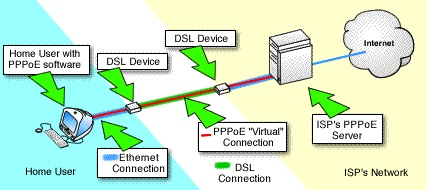
\includegraphics[width=0.5\textwidth]{img/PPP-Visualisierung}
 \caption{Darstellung einer PPP-Verbindung zwischen Heimanwender und ISP (Entnommen aus \cite{PPP-Bild})}
 \label{fig:PPP-Visualisierung}
\end{figure}
Neben DSL-Anschl\"ussen gibt es in Deutschland die Alternative des Kabel-Anschlusses. Bei Kabel-Anschl\"ussen wird nicht das PPP-Protokoll zum Aufbau einer Verbindung genutzt, sondern das DOCSIS-Protokoll zusammen mit einer DHCP-\"ahnlichen \cite{RFC3256} Funktionsweise. 
\section{Section Heading Here}
\section{Kommunikationsabläufe}
Das PPP eignet sich für die Übertragung über eine Vielzahl an Physical Layer Protokollen.
Hierzu zählen unter anderem  Synchronous Optical Network (SONET), GPRS-/UMTS oder auch
in Verbindung mit Ethernet über die weit verbeitete PPPoE-Variante für die Übertragung
über Direct Subscriber Line (DSL) Anschlüsse\cite{IEEEhowto:kopka}.
An dieser Stelle wird exemplarisch der Kommunikationsablauf anhand von PPPoE aufgezeigt.
\subsection{PPP over Ethernet}
Dass PPPoE Protokoll ist in RFC 2516 spezifiziert und wurde ursprünglich
von den Firmen UUNET, Redback Networks und Router Waree ntwickelt \cite{RFC2516}.
PPPoE ermöglicht die Übertragung von PPP-Paketen auf Basis von Ethernet wodurch
die Authentifizierungsfunktionen von PPP mit den
simultanen Zugriffsmöglichkeiten des Ethernet kombiniert werden.
Die Notwendigkeit für PPPoE resultierte aus dem anfang dieses Jahrtausends
einhergehenden Einzugs der DSL-Technologie und der notwendigen Umstrukturierung
der benötigten Software und Hardware. Ziel war es ein Protokoll zu entwickeln
welches die bis dahin vorherrschende Einwahl-Verfahren möglichst Kostengünstig
ersetzt. Mit PPPoE war es einerseits möglich die bis dahin bestehenden Software-Stacks für PPP
mit minimalen Anpassungen weiter zu verwenden und ließ sich andererseits mit einfacher
und damit günstiger Hardware umsetzen\cite{dslapp}.
Eines der Haupteinsatzgebiete von PPPoE sind somit Breitbandzugänge über DSL-Anschlüsse,
Wireless-Zugängen oder Kabelmodems und wird
auch von vielen Internet Service Providern (ISP) zu diesem Zweck eingesetzt \cite[p.88]{cisconut}.\\
%
Der strukturelle Aufbau eines typischen PPPoE-Pakets ist in \ref{fig:PPPoE_Bild} zu sehen.
\begin{figure}[h!]
 \centering
  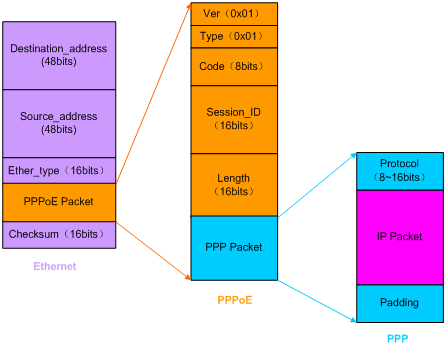
\includegraphics[width=0.5\textwidth]{img/pppoe_aufbau.jpg}
 \caption{Aufbau eines PPPoE-Pakets (Entnommen aus \cite{PPPoE_Bild})}
 \label{fig:PPPoE_Bild}
\end{figure}
Hierbei ist die Verschachtelung der Protokolle der einzelnen Layer zu erkennen: Die unterste
Ebene bildet Ethernet, gefolgt von PPPoE zur PPP bis zum Internet Protokoll.
Der Aufbau von Ethernet und IP-Paketen wird als bekannt vorausgesetzt und hier nicht näher erläutert.\\
%
Die Bedeutung der PPPoE header ist in Tabelle \ref{tab:PPPoE_fields} dargestellt.
%
\begin{figure}[h!]
\begin{tabular}{|l|p{6.5cm}|}
\hline 
Ver & Verwendete Version des PPPoE, immer 1\\ 
\hline 
Type & Verwendeter Typ des PPPoE, immer 1\\ 
\hline 
Code & Typ des PPPoE\-Pakets: 0x00 = Sitzungsdaten; 0x09 = PADI; 0x07 = PADO oder PADT;
0x19 = PADR; 0x65 indicates PADS\\ 
\hline 
Session\_ID & Eindeutiger identifier einer PPP\-Sitzung\\ 
\hline 
Length & Länge des PPPoE\-Payloads\\ 
\hline 
Protocol & Protokolltyp des nächsten Layers\\ 
\hline
\end{tabular}
\end{figure}
% TODO: scheiß label für Tabelle???
\label{tab:PPPoE_fields}
%
Der Ablauf einer PPPoE-Verbindung teilt sich in die drei Phasen Discovery, Session und Terminate
ein. Diese werden in Abbildung in den folgenden Abschnitten näher erläutert (vgl. \cite{RFC2516}).\\
%
\begin{figure}[h!]
 \centering
  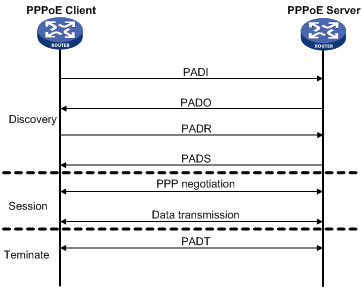
\includegraphics[width=0.5\textwidth]{img/pppoe_sequenz1.png}
 \caption{Ablauf einer PPPoE-Session (Entnommen aus \cite{PPPoE_Bild})}
 \label{fig:PPPoE_sequenz1}
\end{figure}
\subsubsection{Discovery}
Das Ziel dieser Phase ist das Auffinden der MAC-Adresse des Servers (auch Concentrator genannt)
sowie das Ableiten einer PPPoE Session-ID durch den Client (auch Host genannt).
Abhängig von der Topologie können sich mehrere Server im Netzwerk befinden, welche in
dieser Phase durch den Client entdeckt werden. Die discovery-Phase selbst ist Zustandslos, d.h.
auf Seiten aller Kommunikations werden keine Verbindungsinformationen gespeichert.\\
Das erste gesendete PPPoE Active Discovery Initiation (PADI) Paket stellt ein Broadcast
an alle im Netzwerk vorhanden Server dar. Dieses enthält den Namen des vom Client
angefragten Service, auf welches Server mit einem
PPPoE Active Discovery Offer (PADO) Paket antworten. Das Antwortpaket
hat als Zieladresse die des Clients und enthält neben dem Namen des Servers optional
weitere vom Server angebotene Service-Namen. Es folgt ein PPPoE Active Discovery Request (PADR) Paket
mit welchem der Client den von ihm nun gewählten Server und Service unter allen
gefundenen direkt addressiert. Nach erhalt des PADR beginnt der Server mit dem Aufbau
einer PPP Session und bestätigt dies mit einem PPPoE Active Discovery Session-confirmation (PADS) Paket.
Diese enthält auch eine Session-ID welche die folgende Session eindeutig Identifiziert.
\subsubsection{Session}
In der Sitzungsphase erfolgt die weitere Konfiguration der Verbindung, die Authentifikation des
Clients sowie der eigentliche Datenaustausch. Dieser ist im gegensatz zur Discovery und Terminate
Phase PPP spezifischim und im Abbildung \ref{} genauer dargestellt.
%
\begin{figure}[h!]
 \centering
  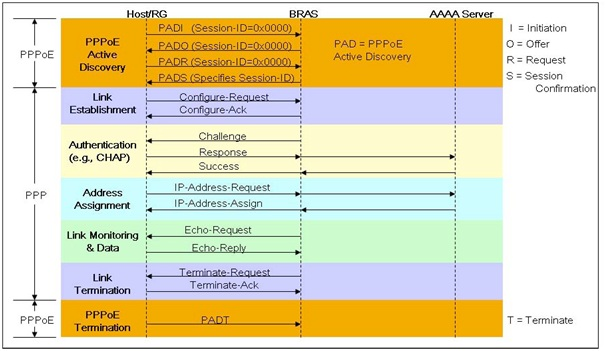
\includegraphics[width=0.5\textwidth]{img/pppoe_sequenz2.jpg}
 \caption{PPP-Spezifischer Teil eines PPPoE-Verbindungsaufbaus (Entnommen aus \cite{pppoe_sequenz2})}
 \label{fig:PPPoE_sequenz2}
\end{figure}
% 
\subsubsection{Terminate}
Die PPPoE Verbindung kann jederzeit von beiden Kommunikationspartner beendet werden. Hierfür sendet
der Client oder der Server ein PPPoE Active Discovery Terminate (PADT) Paket. Nach Erhalt dieses
Pakets ist kein weiterer Datenaustausch über die Session erlaubt.
%
%
\section{Conclusion} 
The conclusion goes here. 
\subsection{Subsection Heading Here} 
Subsection text here. 
% needed in second column of first page if using \IEEEpubid 
%\IEEEpubidadjcol 
\subsubsection{Subsubsection Heading Here} 
Subsubsection text here. 
\appendices 
\section{Proof of the First Zonklar Equation} 
Appendix one text goes here. 
% you can choose not to have a title for an appendix 
% if you want by leaving the argument blank 
\section{} 
Appendix two text goes here. 
% use section* for acknowledgement 
\section*{Acknowledgment} 
The authors would like to thank... 
% Can use something like this to put references on a page 
% by themselves when using endfloat and the captionsoff option. 
\ifCLASSOPTIONcaptionsoff 
  \newpage 
\fi
\begin{thebibliography}{1} 
\bibitem{IEEEhowto:kopka} 
H.~Kopka and P.~W. Daly, \emph{A Guide to \LaTeX}, 3rd~ed.\hskip 1em plus 
  0.5em minus 0.4em\relax Harlow, England: Addison-Wesley, 1999. 
Andrew S. Tanenbaum: Computer Networks, 5.th edition, Prentice Hall, 2011
James F. Kurose / Keith W. Ross, Computernetzwerke, Pearson, 2012

%RFC 1661 – Point-to-Point Protocol (PPP) July 1994;
%RFC 1662 – Point-to-Point Protocol in HDLC-like Framing
%RFC 1962, PPP Compression Control Protocol (CCP)
%RFC 1963, PPP Serial Data transport Protocol
%RFC 1990, The PPP Multilink Protocol (MP)
%RFC 1994, PPP Challenge Handshake Authentication Protocol (CHAP)
%RFC 2153, Informational, PPP Vendor Extensions
%RFC 2284, PPP Extensible Authentication Protocol (EAP)
%RFC 2364, PPP over ATM
%RFC 2516, PPP over Ethernet
%RFC 2615, PPP over SONET/SDH
%RFC 2686, The Multi-Class Extension to Multi-Link PPP
%RFC 2687, Proposed Standard, PPP in a Real-time Oriented HDLC-like Framing
%RFC 5072, IP Version 6 over PPP
%RFC 5172, Negotiation for IPv6 Datagram Compression Using IPv6 Control Protocol
%RFC 6361, PPP Transparent Interconnection of Lots of Links (TRILL) Protocol Control Protocol
\bibitem{RFC2516} A Method for Transmitting PPP Over Ethernet (PPPoE) (IETF RFC2516), \newblock L. Mamakos, \newblock K. Lidl, \newblock J. Evarts, \newblock 1999.
\bibitem{RFC2637} Point-to-Point Tunneling Protocol (IETF RFC 2637), \newblock K. Hamzeh, \newblock The Internet Society, \newblock Juli, \newblock 1999.
\bibitem{RFC1661} Point-to-Point Protocol (IETF RFC 1661), \newblock W. Simpson, \newblock The Internet Society, \newblock Juli, \newblock 1994.
\bibitem{RFC2364} Point-to-Point Protocol over AAL5 (IETF RFC 2364), \newblock  G. Gross, \newblock The Internet Society, \newblock Juli, \newblock 1998.
\bibitem{RFC2516} Point-to-Point Protocol over Ethernet (IETF RFC 2516), \newblock  L. Mamakos, \newblock The Internet Society, \newblock Februar, \newblock 1999.
\bibitem{RFC3256} The DOCSIS (Data-Over-Cable Service Interface Specifications) Device Class DHCP (Dynamic Host Configuration Protocol) Relay Agent Information Sub-option (IETF RFC 3256), \newblock  D. Jones
, \newblock The Internet Society, \newblock April, \newblock 2002.
\bibitem{PPP-Bild} Veranschaulichung einer PPP-Verbindung, \newblock Vicomsoft, \newblock http://www.vicomsoft.com/learning-center/pppoe/
\bibitem{cisconut} Cisco IOS in a Nutshell \newblock James Boney, \newblock O'Reilly Media \newblock 2005
\bibitem{dslapp} Implementation and Applications of DSL Technology, \newblock Philip Golden Hervé Dedieu, \newblock Krista S. Jacobsen, \newblock 1998
%\bibitem{RFC1055} http://tools.ietf.org/html/rfc1055
%\bibitem{PPPoE_Bild} Aufbau eines PPPoE\-Pakets,\newblock H3C \newblock http://www.h3c.com/portal/Products___Solutions/Technology/WAN/Technology_White_Paper/200911/654415_57_0.htm
%\bibitem{pppoe_sequenz1} Ablauf eine PPPoE-Verbindung,\newblock xxx \newblock http://
%\bibitem{pppoe_sequenz2} PPP-Spezifischer Teil eines PPPoE-Verbindungsaufbaus,\newblock xxx \newblock http://
\end{thebibliography} 
\end{document} 
